% Created 2016-09-23 Fri 13:31
\documentclass[12pt,a4]{article}


\usepackage{hyperref}
\usepackage{minted}
\usepackage{fontspec,xltxtra,xunicode}
\setmainfont[Scale=0.9]{Lato}
\setmonofont[Scale=0.7]{Menlo}
\author{Vittorio Zaccaria}
\date{\today}
\title{Some notes on functionalization of mashup composition}
\hypersetup{
 pdfauthor={Vittorio Zaccaria},
 pdftitle={Some notes on functionalization of mashup composition},
 pdfkeywords={},
 pdfsubject={},
 pdfcreator={Emacs 24.5.1 (Org mode 8.3.6)}, 
 pdflang={English}}
\begin{document}

\maketitle
\tableofcontents

\newpage

\section{Background}
\label{sec:orgheadline1}

It is well understood that the CDT model allows for a declarative expression of
the type of a context \(c\) which we will broadly assume to be values/parameters
associated with the situational needs in which the query must be answered.

\vspace{0.25cm}
\begin{figure}[htb]
\centering
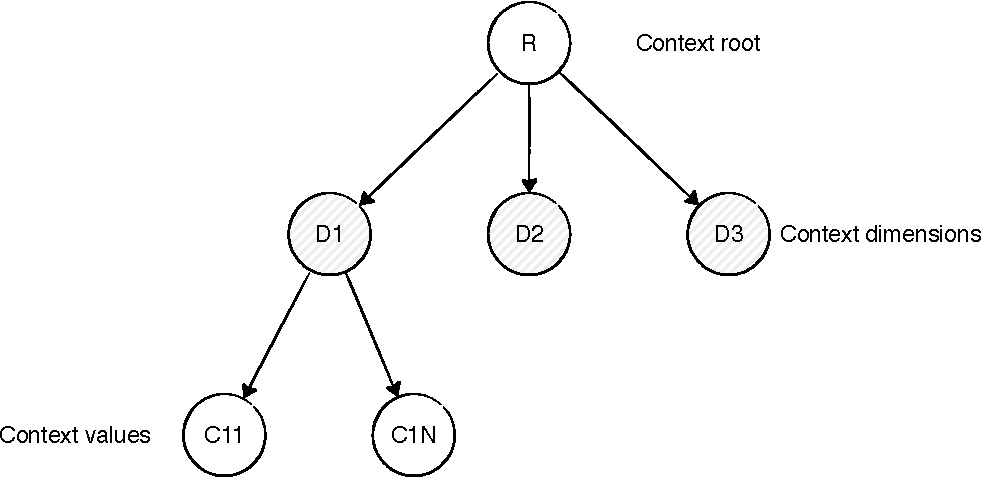
\includegraphics[width=8cm]{./key/page-1-crop.pdf}
\end{figure}
\vspace{0.25cm}

Each dimension \(D_d\) has one value of type indicated by one of children
\(C_{d,i}\), also called \textbf{conceptual nodes}. 

Each children \(C\) can have one or more parameters and provides a \textbf{view}, i.e. some way of
extracting interesting data from a particular data store (being it a database or
a online service). 

\newpage

\section{Operation implementation}
\label{sec:orgheadline5}

Let us try to produce an implementation of the following CDT:

\vspace{0.25cm}
\begin{figure}[htb]
\centering
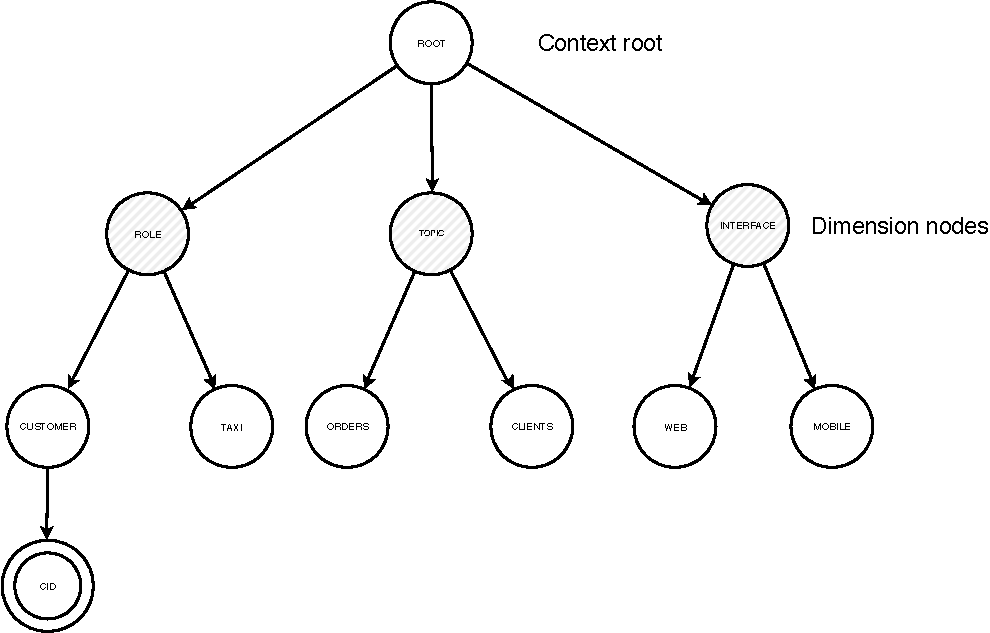
\includegraphics[width=8cm]{./key/page-2-crop.pdf}
\end{figure}
\vspace{0.25cm}

We can identify the following dimensions which can be seen as instances of an enumerative type: 

\begin{minted}[obeytabs=true,baselinestretch=0.95]{haskell}
data Dimension   = Role | InterestTopic | Interface
\end{minted}

and the following concepts:

\begin{minted}[obeytabs=true,baselinestretch=0.95]{haskell}
data Concept = Customer Int
               | Restaurant
               | Orders Int
               | Food 
               | Web 
               | SmartPhone
\end{minted}

Finally we define a context as an array of concepts with their own values:

\begin{minted}[obeytabs=true,baselinestretch=0.95]{haskell}
data Context     = Ctx [ Concept ] deriving (Show)
\end{minted}

\subsection{Describing the tree}
\label{sec:orgheadline2}

We can thus see the CDT as a tree of nodes (\texttt{Tree NodeData}), where each node can
be one of three things:

\begin{minted}[obeytabs=true,baselinestretch=0.95]{haskell}
data NodeData    = D Dimension | C (Context -> Maybe View) | Root
\end{minted}

Each node, in fact, associates a concept with a view which we implement as a
function (\texttt{Context -> Maybe View}). For example, the node associated with the
\texttt{Customer} concept looks in the context to see whether there is a request for a
specific context value; in our example queries are just sql-like strings:

\begin{minted}[obeytabs=true,baselinestretch=0.95]{haskell}
customerView :: Context -> Maybe View
customerView (Ctx []) = Nothing
customerView (Ctx (Customer n:_)) = Just $ E $ "select customers where id=" ++ show n
customerView (Ctx (_:xs)) = customerView (Ctx xs)
\end{minted}

\subsection{Working with the tree}
\label{sec:orgheadline3}

First of all, we should define views as a monoid with a unit (\texttt{mempty}) and an
operator (\texttt{mappend}) to join them; in our case the operator joins query strings:

\begin{minted}[obeytabs=true,baselinestretch=0.95]{haskell}
instance Monoid View where
  mempty              = Empty
  mappend Empty x     = x
  mappend y Empty     = y
  mappend (E x) (E y) = E (x ++ " doubleintersection " ++ y)
\end{minted}

The actual view creation can be seen as a \texttt{fold} operation of views that each
concept node generates given the current context. In the following, function \texttt{f}
is used to transform each node into either a valid view or the empty view.  

\begin{minted}[obeytabs=true,baselinestretch=0.95]{haskell}
getViews :: Foldable t => Context -> t NodeData -> View
getViews ctx = foldMap (f ctx) where 
    f cx (C c)  = fromMaybe mempty (c cx) 
    f _         = mempty
\end{minted}

\subsection{Example operation}
\label{sec:orgheadline4}

Given:

\begin{minted}[obeytabs=true,baselinestretch=0.95]{haskell}
context = Ctx [ Web, Customer 3 ]
cdt = Node Root [
        dim Role [ leaf customerView ],
        dim InterestTopic [],
        dim Interface [ leaf webView ]
  ]
\end{minted}

getting the views gives:

\begin{verbatim}
λ> getViews context cdt
E "select customers where id=3 doubleintersection select _ where type=web"
\end{verbatim}
\end{document}